\documentclass[a4paper,11pt]{kth-mag}
\let\ifpdf\relax
\usepackage[T1]{fontenc}
\usepackage{textcomp}
\usepackage{lmodern}
%\usepackage[latin1]{inputenc}
\usepackage[swedish,english]{babel}
\usepackage{modifications}
\usepackage{amsmath}
\usepackage{ifpdf}
\usepackage[breaklinks=true]{hyperref}
\usepackage{breakcites}
\usepackage{pdfpages}

\newcommand{\textunderscript}[1]{$_{\text{#1}}$}
\usepackage[utf8]{inputenc}
%\usepackage{cite}
%\usepackage{biblatex}
%\addbibresource{references.bib}
%\newenvironment{italicquotes}
%{\begin{quote}\itshape}
%{\end{quote}}

%% Graphic packages
\usepackage{graphicx}
\usepackage{tikz}
\usepackage{tikz-3dplot}
\usetikzlibrary{positioning}
\usepackage{circuitikz}
\usetikzlibrary{calc,patterns,decorations.pathmorphing,decorations.markings}
\usepackage{subcaption}
\usepackage{tikz-cd}
\usetikzlibrary{decorations.text}

\tikzset{
    %Define standard arrow tip
    >=stealth',
    %Define style for boxes
    punkt/.style={
           rectangle,
           rounded corners,
           draw=black, very thick,
           text width=6.5em,
           minimum height=2em,
           text centered},
    % Define arrow style
    pil/.style={
           ->,
           thick,
           shorten <=2pt,
           shorten >=2pt,}
}




%\usepackage{appendix} 
\title{The Black Box}
\subtitle{Control and design of reaction wheel based inverted pendulum}
\foreigntitle{Stabilisering med svänghjul Utevkcla...}
\author{Mikael Sjöstedt \\ Alexander Ramm}
\date{May 2015}
\blurb{ Bachelor's Thesis in Mechatronics \vspace{1em} \\
\begin{tabular}{ll} 
Supervisor: Daniel Frede &  \\
Examiner: Martin Edin Grimheden \\ 
Approved: TBA 2015-month-day
\end{tabular} }
\trita{TRITA xxx yyyy-nn}


\begin{document}


\includepdf[pages={1}]{kth-cover.pdf}
\clearpage

\frontmatter
\pagestyle{plain}
%\removepagenumbers
\pagenumbering{roman}
\maketitle
\selectlanguage{english}
\begin{abstract}
\addcontentsline{toc}{chapter}{Abstract}
Robots that move require a high degree of precision from position tracking sensors. This paper studies how the 
placement of these sensors effect the robots ability to determine its position. A robot with a cubical frame is
built, which were able to balance on a edge with help of a reaction wheel. The robot determined its rotation using an inertial measurement unit. Different sensor positions were evaluated empirically and...

\textbf{More selling from beginning. Dont miss results and conclusions}
 
\end{abstract}
\cleardoublepage
\begin{foreignabstract}{swedish}
\addcontentsline{toc}{chapter}{Sammanfattning}
Robotar som förflyttar sig kraver mycket precis nogrannhet från sina positionerings sensorer. Det här rapporten tar
upp hur placeringen av dessa sensorer påverkar robotens förmåga att bestämma sin position. Från en kubformad ram 
byggdes en robot, som med hjälp av ett motordrivet svänghjul kan applicera ett internt moment för att balansera på en kant. Roboten använde en sensor av typen --inertial measurment unit-- för att bestämma sin position. Olika placeringar av sensorn utvärderases empiriskt och ...
\\


%Examensarbetet skrivs på engelska och har alltid både en svensk och en engelsk sammanfattningssida. Denna skrivmall, som inte har ``bookmarks'' eller några avancerade ``features'', definierar layouten för ett examensarbete i Maskinteknik (MF123X) eller Industriell ekonomi (MF105X).
%I detta kapitel sammanfattas examensarbetet. Sammanfattningens omfattning är högst en sida. Sammanfattningen åtföljs av en blank sida. Den föregående titelsidan, som lämpligen också innehåller en illustrativ bild, följs också av en blank sida. Alla kapitel börjar längst upp på en högersida, dvs på ett udda sidonummer.
\end{foreignabstract}
\clearpage
\chapter*{Preface}
\addcontentsline{toc}{chapter}{Preface}
Here goes our thanks to sources of  help, cooperation, inspiration \\ To be filled in \\
% Here goes credits to Daniel Frede, Staffan, Assarna som tog sig tid, eventuella maskiner som inte strulat
\begin{flushright}Alexander Ramm \\Mikael Sjöstedt \\ KTH, månad, 2015 \end{flushright}

% We would like to thank our supervisor Daniel Frede for his continous --- and could point us in the right direction. osv osv 

%\clearpage


\cleardoublepage
\addcontentsline{toc}{chapter}{Contents}
\printindex
\tableofcontents*

\cleardoublepage
\chapter*{Nomenclature}
\addcontentsline{toc}{chapter}{Nomenclature}
\section*{Symbols - needs restructure}
\noindent{}\begin{tabular}{@{}p{2.5cm}l}
\textbf{Symbol} 	& \textbf{Description} \vspace{.5em} \\
$E$ 		& Elasticity module (Pa) \\
$r$		& Radius (m) \\
$t$		& Thickness (m) \\
$\mathcal{L}$			& Lagrange \\
$\theta$		& Cube angle\\
$\phi$		& Flywheel angle \\
$q$			& Lagrange operator \\
$E_k	$		& Kinetic energy \\
$E_p$		& Potential Energy \\
$I_c$		& Inertia of the cube\\
$I_f$		& Inertia of the flywheel\\
$M\textsubscript{tot}$		& Total mass of the cube\\
$M_f$		& Mass of the flywheel \\
$i$			& Current\\
$K_t$		& Motor torque constant\\
E\textunderscript{emf} 	& Induced voltage \\
K\textunderscript{emf} 	& Motor voltage constant \\
U			& Voltage across motor poles\\
$R_m	$		& Motor internal resistance \\
$\eta_m$		& Motor efficiency\\	
$\eta_g$		& Gear efficiency \\
$u$			& Gear ratio\\
$z$			& Measurement noise \\
$w$			& Process noise \\

\end{tabular}
\clearpage

\section*{Abbreviations}
\noindent{}\begin{tabular}{@{}p{2.5cm}l}
\textbf{Abbreviation} 	& \textbf{Description} \vspace{.5em} \\
CAD			& Computer Aided Design \\
CAE			& Computer Aided Engineering\\
PLM			& Product Lifecycle Management\\
PWM			& Pulse With Modulation\\
DOF			& Degrees of freedom\\
MEMS			& Microelectromechanical Systems \\
MATLAB		& Matrix Laboratory, computational program\\
RMS			& Root Mean Square\\
MCU			& Microcontroller\\
IC			& Integrated circuit\\
$I^2C$		& Inter-Integrated circuit\\
USB			& Universal Serial Bus \\
UAV			& Unmanned Aerial Vehicle\\
\end{tabular}
\cleardoublepage

\mainmatter
\pagestyle{newchap}

\chapter{Introduction}
This chapter describes the background, purpose and scope of this project conducted at the mechatronics department at the Royal Institute of Technology, KTH, Sweden. The work was carried out during the spring 2015.

\section{Background}
A reaction wheel is a wheel that is accelerated to apply torque. The most wide spread use of reaction wheels is in human made satellites. The  reaction wheels, usually three of them in the case of satellites, are used to change the attitude of the satellite by applying torque in a favourable manner. This is imperative to direct solar panels towards the sun or pointing antennas to assure maximum performance and connectivity to the satellite. Compared \textbf{to most} machines satellites are quite uncommon (there are ~1100 satellites currently in orbit [source]), and their technology can at times seem alien. But reaction wheels should not be alienated, they can be used in many contexts and this paper will cover one of them.  

Balancing 1 \textit{degree of freedom} (DOF) inverted pendulum type structures using reaction wheels is no
new concept, and became more accessible with the introduction of cheap microcontrollers.
The use of automated control is growing at a rapid pace and is being implemented
more and more in consumer related products.  This growth
has made automated control together with sensors available more now than ever. It can be seen in the every-day life in product lines such as mobile phones, gaming controllers, cars and UAVs such as quadrocopters.

One of the most basic systems that requires some control to become stable is the inverted pendulum. 
Although it is simple to define, its control is not. A lot of work has been done on the topic
but there are still no knowledge easily acquired by the \textbf{public available??}. 

The method to achieve balance of the pendulum using reaction wheels is even more narrow. 
In recent years prototypes of land based structures using reaction wheels have been a hot topic and some of these robots are truly remarkable. 

\textbf{pretty shady part. Maybe to the authors it would be a great achievment. medel på det där med PHD }
It would be a great achievement to contribute knowledge about how such a mechanism could be built and evaluate
the capabilities and restrictions of such a machine, on a level that does not require a PhD.


\section{Purpose}
The goal of the project was to build a structure with one degree of freedom that can maintain balance using a reaction wheel and examine the behaviours of the system. A concept idea of the robot can be seen in Figure \ref{Figure: concept idea}
\begin{figure}[!htb] 
\centering
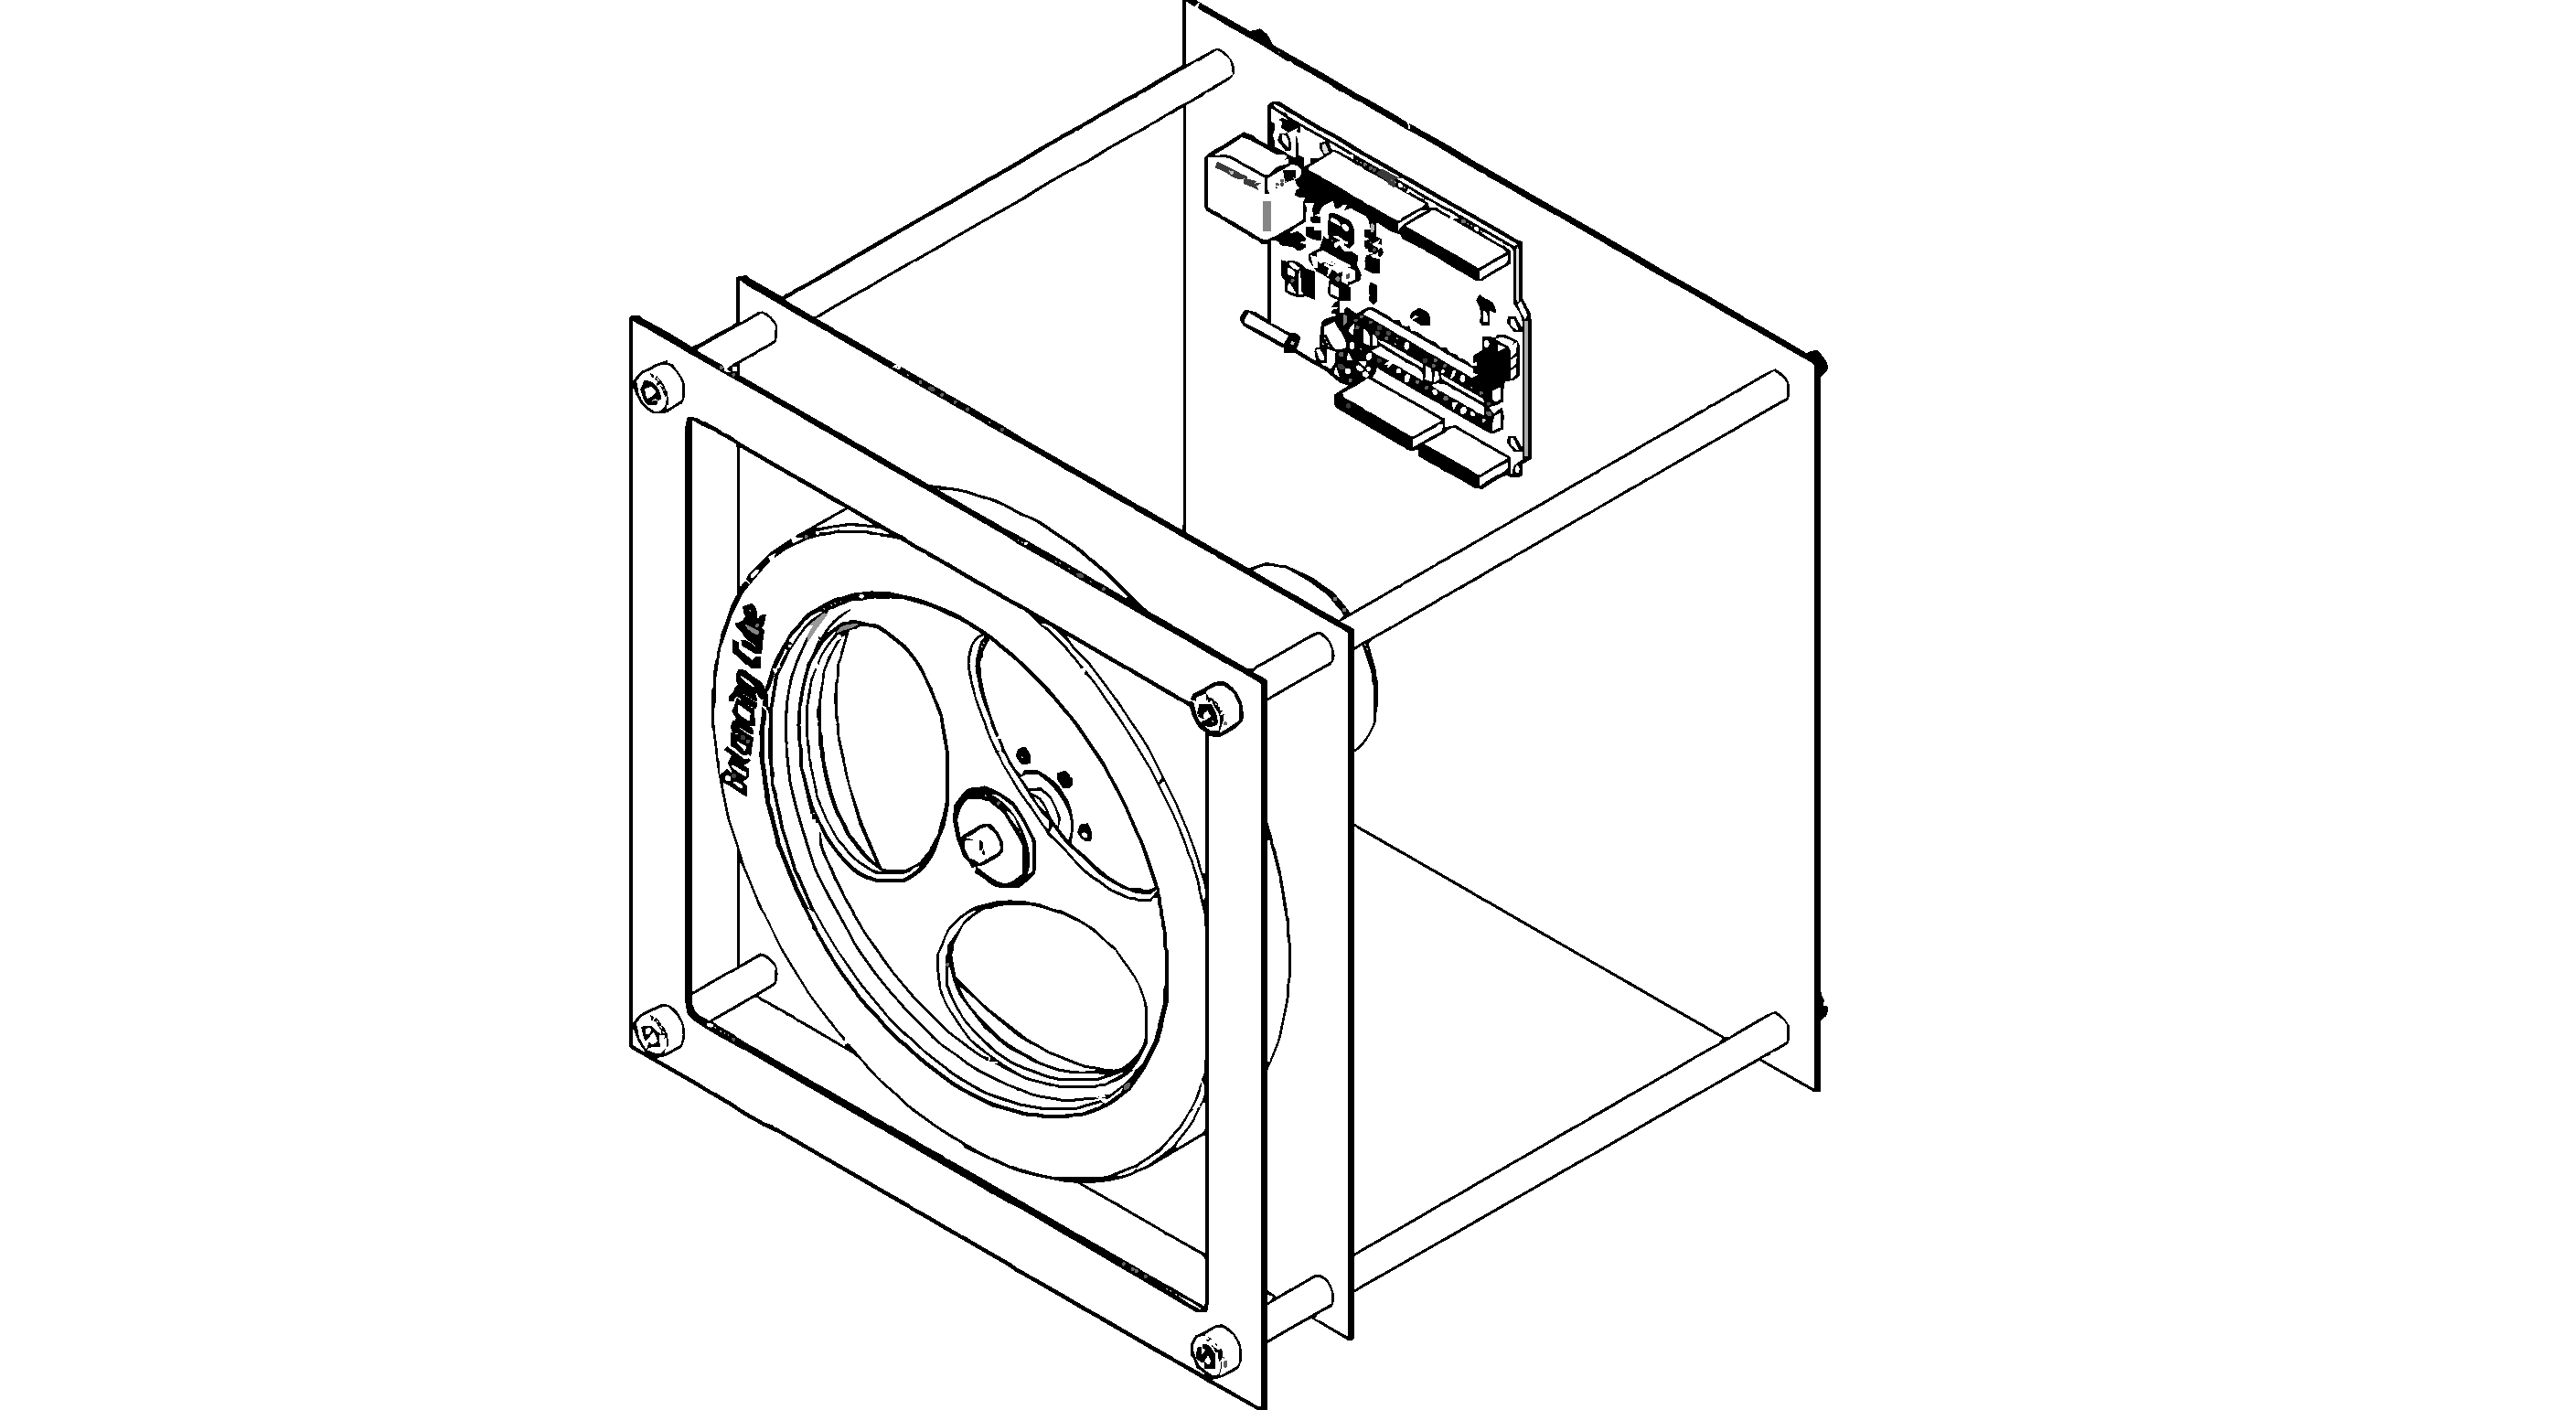
\includegraphics[width = \textwidth]{concept.pdf}
\caption{Concept design}
\label{Figure: concept idea}
\end{figure}

The dynamics is mostly effected by the control system, which is responsible for accelerating the motor in the  correct angular direction, to maintain balance. The parameters in the control system effects response time, overshoot and sinusoidal settling time.
This project will hopefully contribute to some development within the open-source community.
All results are available online, open source (MIT license reference here), on GitHub \cite{Github}.
As a thesis in mechatronics, this paper can be divided into two parts. One engineering part whose focus to implement knowledge in mechanics, electronics and control theory to result in a functioning robot. A research part whose topic could be concentrated to a question 

\begin{quote}
\textit{
How does the sensor placement effect the quality of the sensor data. --- what is quality ? how it effects system performance?}
\end{quote}
The only sensor that can be placed arbitrarily in the system is the \textit{Inertial Measurement Unit} (IMU). Certain positions might have an advantage in terms of how usable the raw data is. The IMU is a sensitive devise and disturbances such as high current and fast oscillations in its vicinity might ruin the data entirely.[citation PLZ]. With quality defined as the usability of the data given by the sensor. \textbf{somewhat vague}

\section{Scope}
The only sensor whose position is to be examined is the IMU, as the encoder for the motor is fixed to the motor shaft and was not examined. Only a few key positions of the sensor were examined.

The effects that were looked at were the ones related to the control system. Mainly the overshoot behaviour and the settling time of the system. Only data used for the specific control system were examined, \textbf{other DOF measurements were not taken into consideration ???}. I.e. \textbf{its a consquence} the results may only be applicable in similar machines and not in general.

For every position the same parameters and constants were used in all systems and software. The comparisons were made in between measurements while balance was maintained and no external disturbance is applied. All measurements where taken during a limited time frame (We dont know this yet....).  \textbf{this might belong to method?}

\section{Method}
The sensor was placed in the upper corner, one of the side corners, between the mentioned corners and in the center of the cube (insert figure reference). Both raw data and filtered data were collected and sent over serial to a computer. Using Matlab \cite{MATLAB:2014} the readings where analysed for stablization behaviour. Other obvious observations were noted. To have equal conditions, all measurements were made on the same horizontal space with the same external voltage supply.

New TRY
The cube was placed in a position close to its upper equlibriub point.
\chapter{Theory}
This chapter cover some of the theory that is required if one want to build a similar robot. It is assumed that the reader has some understanding of Newtonian mechanics, signal analysis and control theory. Basic understanding of DC motor operation is also an advantage.

The first part is about the inertial reference unit that covers issues of sensor characteristics and why they are important to the system as a whole and the research question in particular.

There is a part that discuss Kalman filter theory, a filter required for getting high quality data from the IMU. The filter interprets noisy data from the sensor and digitally filters the signal to a more trustworthy output. 

The last part covers the theory of the mechanical system behaviour that is used to develop the state space control system. The equations are responsible for the actual balance part and thus important. 

% When using a sensor such as an IMU one can choose between different resolution settings, depending of the specific usage. Although the resolutions were not changed between measurements these settings could be important when comparing to another machine


\section{Inertial Measurement Unit} \label{section:IMU}
\subsection{Background}
The data collected for calculating the angle of the cube is gathered from an IMU, a unit that uses both an accelerometer and a gyroscope to track the orientation and position. A IMU is often rated for several \textit{degrees of freedom} (DOF), a unit specified as 6-DOF uses three orthogonal accelerometers and gyroscopes. These measure linear acceleration and angular velocity respectively. There are also units that are rated for additional degrees of freedom and usually include features such as magnetometer or barometer sensors.   
To understand the fundamentals of an inertial system a Cartesian coordinate system is defined in Figure \ref{Figure: cartesian}

\begin{figure}[!hbt] 
\centering
\tdplotsetmaincoords{60}{110}
%
\pgfmathsetmacro{\rvec}{.8}
\pgfmathsetmacro{\thetavec}{30}
\pgfmathsetmacro{\phivec}{60}
%

\begin{tikzpicture}[scale=6,tdplot_main_coords]
    \coordinate (O) at (0,0,0);
    \draw[thick,->] (0,0,0) -- (1,0,0) node[anchor=north east]{$x$};
    \draw[thick,->] (0,0,0) -- (0,1,0) node[anchor=north west]{$y$};
\draw[thick,->] (0,0,0) -- (0,0,1) node[anchor=south]{$z$};
	\node at (0.5,0,0) (x) {};

\tdplotdrawarc[->,color=black]{(0,0,0.6)}{0.1}{0}{340}{anchor=south west,color=black}{yaw}
%We move to the z-x axis
\tdplotsetthetaplanecoords{0}

\tdplotdrawarc[tdplot_rotated_coords,->,color=black]{(0,0,0.6)}{0.1}{110}{450}{anchor=south west,color=black}{pitch}
\tdplotsetthetaplanecoords{-90}

\tdplotdrawarc[tdplot_rotated_coords,->,color=black]{(0,0,0.6)}{0.1}{120}{460}{anchor=south west,color=black}{roll}

\end{tikzpicture}
\caption{Cartesian coordinate system}
\label{Figure: cartesian}
\end{figure}
 
 --The accelerometer is used to measure the acceleration along the lines of $x,y,z$ axes while the gyroscope measures the angular rate around these axes, ie if the gyroscope rotates along the $z$-axis it would output a yaw rate.--  \textbf{Unnecessary ?}
 
The inertial navigation system used in this project is a small \textit{microelectro-mechanical system} (MEMS). A micromechanical sensor is a very small unit that make use of its mechanical properties to sense alteration in the environment \cite{ref:accelerometero}. The advantages of these small units are low production costs, small size and low power consumption. As the research of these fairly modern units continues the reliability increases but the raw output still contains significant noise \textbf{medel på denna mening, raw output vafan kom på något innovativt}. \cite{IMUintro}
\subsection{Accelerometer} \label{sec: accelerometer}
Accelerometers are used to measure linear acceleration. Or rather, it measure forces due to acceleration. These forces can be divided into two groups
\begin{itemize}
\item Static forces, such as gravity
\item Dynamic forces, due to movement
\end{itemize}
The force is then converted into acceleration, this is done by measuring the change in capacitance when a spring mass system is moving. The typical accelerometer consists of a movable mass that is attached via a mechanical spring or suspension system to a frame that is used as reference. 
The capacitance is usually measured between a conductive plate and the known mass, seen in figure \ref{Fig: Accelerometer}. The capacitance is then used to determine the displacement of the mass and then calculate the force applied to it with the known spring mass system.

\begin{figure} [!hbt]
\centering
\begin{tikzpicture} [every node/.style={draw,outer sep=0pt,thick},]

\tikzstyle{spring}=[thick,decorate,decoration={zigzag,pre length=0.3cm,post length=0.3cm,segment length=6}]
\tikzstyle{damper}=[thick,decoration={markings,  
  mark connection node=dmp,
  mark=at position 0.5 with 
  {
    \node (dmp) [thick,inner sep=0pt,transform shape,rotate=-90,minimum width=15pt,minimum height=3pt,draw=none] {};
    \draw [thick] ($(dmp.north east)+(2pt,0)$) -- (dmp.south east) -- (dmp.south west) -- ($(dmp.north west)+(2pt,0)$);
    \draw [thick] ($(dmp.north)+(0,-5pt)$) -- ($(dmp.north)+(0,5pt)$);
  }
}, decorate]
\tikzstyle{ground}=[fill,pattern=north east lines,draw=none,minimum width=0.75cm,minimum height=0.3cm]



\begin{scope}[]
\node (M) [minimum width=1cm, minimum height=2.5cm] {$m$};

\node (ground) [ground,anchor=north,yshift=-0.25cm,minimum width=1.5cm] at (M.south) {};
\draw (ground.north east) -- (ground.north west);
\draw [thick] (M.south west) ++ (0.2cm,-0.125cm) circle (0.125cm)  (M.south east) ++ (-0.2cm,-0.125cm) circle (0.125cm);

\node (wall) [ground, rotate=-90, minimum width=3cm,yshift=-3cm] {};
\draw (wall.north east) -- (wall.north west);

\draw [spring] (wall.170) -- ($(M.north west)!(wall.170)!(M.south west)$);
\draw [damper] (wall.10) -- ($(M.north west)!(wall.10)!(M.south west)$);

\node (arrow) [draw=none, above right = -0.5cm and 0 cm of M, label={[xshift=0.7cm, yshift=0cm] $\Delta$ C}] {};
\draw [<->,thick] (arrow) ++ (0.2cm,0) -- +(1cm,0);

\end{scope}

%\draw[step=1cm,gray,very thin] (-2,-2) grid (6,6);
\draw [thick] (2.2,-1.3) -- (2.2,1.3);
%\node (wall2) [thick,rotate = 90, minimum width = 3cm, xshift = 0cm, yshift = -2.5cm] {};
%\draw [thick] (wall2.east) -- (wall2.east);
 


\end{tikzpicture}
\caption{Accelerometer capacitance }
\label{Fig: Accelerometer} 
\end{figure}

Typical noise sources in accelerometers are mechanical vibration of the springs, circuitry and general equipment disturbances. The accelerometer in this project is used to cross-check the perceived angle by the gyroscope, i.e. the signal has to be integrated to calculate an angle. \textbf{omskrivning?}-- A \textbf{measure} to specify how much the noise effects the integrated value is represented 
by the \textit{velocity random walk} (VRW) \cite{ARW}. The signal from the accelerometer during a stationary position can be characterized as a white noise, and the integrated value is going to "walk" around the mean value, hence the name \textit{random walk}.
The accelerometer also outputs a bias, it is essential to determine the bias when estimating a position otherwise the error would grow quadratic due to multiple integration of the measurements \cite{ref:accelerometero}.

\subsection{Gyroscope} \label{gyroscope}
Gyroscopes unlike accelerometers, do not measure linear acceleration. Gyroscopes measure the angular velocity. This is done by making use of the Coriolis effect to measure the angular rate.

\begin{figure}[!hbt]

\centering

\tdplotsetmaincoords{60}{110}

%

\pgfmathsetmacro{\rvec}{.8}

\pgfmathsetmacro{\thetavec}{30}

\pgfmathsetmacro{\phivec}{60}

%

\begin{tikzpicture}[scale=8.5,tdplot_main_coords]

    \coordinate (O) at (0,0,0);

    \draw[thick,->] (0,0,0) -- (0.7,0,0) node[anchor=north east]{$x$};

    \draw[thick,->] (0,0,0) -- (0,0.7,0) node[anchor=north west]{$y$};

\draw[thick,->] (0,0,0) -- (0,0,0.7) node[anchor=south]{$z$};

	\node at (0.5,0,0) (x) {};



%The cube

\draw (0.2, 0.5,0.5) -- (0.2,0.5,0.6) -- (0.2,0.4,0.6) -- (0.3,0.4,0.6) -- (0.3,0.4,0.5) -- (0.3, 0.5, 0.5) -- (0.2,0.5,0.5)--(0.2,0.5,0.6)--(0.3,0.5,0.6)--(0.3,0.4,0.6)--(0.3,0.5,0.6)--(0.3,0.5,0.5);





\draw [->] (0.25,0.5,0.55) -- (0.25,0.65,0.55) node[anchor = north east] {$v$};



\draw [->] (0.3,0.45,0.55) -- (0.45,0.45,0.55) node[anchor = south east] {$F_c$};



%\tdplotdrawarc[->,color=black]{(0,0,0.5)}{0.05}{0}{-330}{anchor=south west,color=black}{\textbf{$\omega$}}

\tdplotsetthetaplanecoords{0}



\tdplotdrawarc[thick, -> ,color=black]{(0.35,0.49,0.75)}{0.06}{0}{-330}{anchor=south west,color=black}{\textbf{$\omega$}}



\end{tikzpicture}

\caption{Gyroscope pic }
\label{Fig: Gyroscope}
\end{figure}

Consider figure \ref{Fig: Gyroscope} where a mass is vibrating along the $y$-axis, with the momentary velocity $v$. When the mass is rotated along the $z$-axis with the angular velocity $w$, a secondary vibration perpendicular to the first is induced which is explained by the Coriolis force
\begin{equation}\label{eq:coriolis}
\textbf{F}_c = -2m(\textbf{\textit{w}} \times \textbf{\textit{v}})
\end{equation}
The result is a physical displacement and a capacitance is measured just like the accelerometer. ---If, for example a rotation occurs along the x-axis the gyroscope would output a \textit{roll} rate. \textbf{not necessary right?}---

A micromechanical gyroscope is, like the accelerometer, effected by a bias. This is often due to friction caused by moving parts or production variations induce stress on the construction resulting in an offset of the output. If a constant error is integrated the angular error grows linearly with time. This is easily corrected by subtracting the bias from the output.
This approach has a drawback. The small size and sensitivity of this device make the bias wander due to flickering noise in the electronics \cite{IMUintro}. Thus a \textit{bias stability} is introduced as a measurement of how the bias may change during a period of time.
Other troublesome errors that occur in MEMS gyroscopes are thermo-mechanical white noise similar to noise in an accelerometer. To indicate how this noise effects the integrated value an \textit{Angle Random Walk} (ARW) is introduced. The ARW is of the same significance as the VRW mentioned in section \ref{sec: accelerometer} but considers the angular velocity instead. \textbf{var kritisk} 

The concepts of ARW, VRW and bias stability that has been introduced are more or less an indication of how precise the measurement devices are.

\section{Kalman filter}
\subsection{introduction}
The signal from an IMU contains data of angular velocities and acceleration, but also a lot of noise, as explained earlier. A position estimated from an untreated signal from an IMU could work for short periods, but over time the estimated position \textit{drifts} \cite{MEMSdrift}. This drift occurs when measurements containing noise is integrated to acquire a position, the readings contain both white noise and often a bias which is making the  error to grow for every calulation.
Integrating the angular motion from the gyroscope to estimate a position would result in an angular drift and an even worse drift for the accelerometer as it is integrated twice to estimate a position.
By using a Kalman filter the drift can effectively be minimized. If the readings from both the gyroscope and accelerometer is considered, and with some help of probablity theory the estimated state is not far from the true value.  A Kalman \textit{filter} is not what the name suggests, it is an estimator. Old and new measurements are processed real-time to calculate an estimation of the current state. 

One could say that the Kalman filter moves between \textsc{two phases (no good)} see Figure \ref{Fig: Kalman phases}. Firstly it estimates a state using a known process, which usually contains a noise. Then it adjusts the state to a measurement.

\begin{figure}
\centering

\begin{tikzpicture}[ auto,]
 \node[xshift = 3cm] (b) {\textbf{Measurement phase}}; 
 \node[xshift = -3cm] (a) {\textbf{Update phase}};
 \node[xshift = 4.5cm, yshift = 1.5cm] (dummy1) {Measurement};
 \node[xshift = -4.5cm, yshift = -1.5cm] (dummy2) {State estimate};
 \draw [->] (a) to [bend left = 45] (b);
 \draw [->] (b) to [bend left = 45] (a);
 \draw [->] (a) to (dummy2);
 \draw [->] (dummy1) to (b);
 
\end{tikzpicture}
\caption{Kalman phases}
\label{Fig: Kalman phases}
\end{figure}

Keep in mind that there are some regards that should be taken into consideration when choosing an estimator.
A good estimator produces states that are non biased, \emph{values that have an average  of the true value}. As well that the estimated state variance from the true state is as small as possible\cite{Simon2001}.


\subsection{State Estimator}
The Kalman filter is, as stated above, is a state based estimator. By using the last measurement and the one before that it can derive a better estimate of the current state. The true state and the measured value at a time \textit{k} would be
\begin{equation}\label{eq:kalmanstate}
x_k = Ax\textsubscript{k-1}+Bu\textsubscript{k-1}+w\textsubscript{k-1}
\end{equation}
\begin{equation} \label{eq:kalmanmeas}
z_k = Hx_k + v_k
\end{equation}
The true state $x$ is expressed with the the old state and an input $u$. But the signal also contains a process noise $w$. The process noise $w$ in equation \eqref{eq:kalmanstate} is a representation of variances in the process that cannot be mathematically predicted. When using a gyroscope this reflects the error characteristics mention in section \ref{gyroscope}. 
The measured value, $z$ seen in equation \eqref{eq:kalmanmeas} is an observed measurement. Ideally this would only be a function of $x$, but is distorted by the measurement noise $v$.
The measurement noise, $v$, much like the process noise is common in any measurement and represents various fluctuations caused by the equipment.
\\ \\
The Kalman filter estimates a reliable state $\hat{x}_k$
\begin{equation}
\hat{x}_k = \hat{x}^-_k + K_k\tilde{y}_k
\end{equation}
where $\hat{x}^-_k$ is an estimation of the state using the process, in this case the gyroscope. The second term $K_k\tilde{y}_k$ contains $\tilde{y}_k$ which is a \textbf{parameter} that consider the measurement, the accelerometer. It also contains the Kalman gain, $K_k$ which indicates how reliable the measurement is and how much it should effect the new estimated state

For further reading and explanation of how the Kalman filter works, see appendix \ref{app: Kalman}.

\textbf{Här bryter jag}




%
%To understand this recursive filter which use old and new values a \textit{a priori} and \textit{a posteriori} state is defined
%\begin{equation} \label{eq: priori state}
%\hat{x}^-_k
%\end{equation}
%\begin{equation} \label{eq: posteriori state}
%\hat{x}_k
%\end{equation}
%The \textit{a priori}  state in equation \eqref{eq: priori state} is defined as the estimate of the current state at the time $k$. The \textit{a posteriori} state \eqref{eq: posteriori state} is the new estimated state.
%For the Kalman filter to work properly some criteria has to be fulfilled. The average value of the measurement noise $z$ and process noise $w$ has to be zero, i.e. a Gaussian error. $z$ and $w$ also has to be independent of  each other. The noise and error in an IMU and many other devices have the characteristics of Gaussian noise.
%
%
%
%
%During the \textit{predict} phase the filter estimates the states using the inputs from the process, i.e the gyroscope. It then moves on to the \textit{update} phase where it compares the state to the actual measurement, the accelerometer. See Figure \ref{Fig: Kalman phases}.
%Consider the true state equation \eqref{eq:kalmanstate}, the Kalman filter is firstly estimating the first state by neglecting the process noise
%\begin{equation} \label{eq:Kalman first estimate}
%\hat{x}^-_k = A\hat{x}\textsubscript{k-1}+Bu\textsubscript{k-1}
%\end{equation}
%As stated above the Kalman filter uses readings from both the gyroscope and accelerometer to estimate a position closer to the true value. To determine how reliable the process and measurement readings are a noise covariance is defined as
%\begin{equation} \label{eq:covariance process noise}
%Q = E(w_k w_k \textsuperscript{T})
%\end{equation}
%\begin{equation} \label{eq:covariance measurement noise}
%R = E(v_k v_k \textsuperscript{T} )
%\end{equation}
%How to determine these covariances are further investigated in section  \ref{chapter:Allan Variance}
%From here the \textit{a priori} error covariance matrix is introduced to symbolize the noise in the process measurement
%\begin{equation}
%P^-_k = AP\textsubscript{k-1}A^T + Q_k
%\end{equation}
%During the \textit{update} the accelerometer measures are used. The measurement \textit{innovation} is calculated as
%\begin{equation} \label{eq: innovation}
%\tilde{y} = z_k - H\hat{x}^-_k
%\end{equation}
%The \textit{innovation} is a residual that reflects the relation between the predicted measurement and the actual measurement. A measurement \textit{innovation} of zero indicates a perfect agreement.
%The measurement \textit{innovation} covariance is calculated as
%\begin{equation} \label{eq:innovation cov}
%S_k = HP^-_kH^T + R
%\end{equation}
%The \textit{innovation} covariance is very similiar to the \textit{priori} error covariance but represents the measurement instead. From here the core of the Kalman filter can be calculated, the Kalman gain
%\begin{equation} \label{eq:Kalman gain}
%K_k = P^-_kH^TS\textsuperscript{-1}_k
%\end{equation}
%indicates how reliable the measurement is. Note that if the measurement covariance error \eqref{eq:covariance measurement noise} is large the Kalman gain will be small and vice versa if the \textit{priori} error covariance is large.
%By now the \textit{posteriori} state can be estimated by
%\begin{equation}
%\hat{x}_k = \hat{x}^-_k + K_k\tilde{y}_k
%\end{equation}
%A current state has been estimated and the Kalman filter and finally the \textit{priori} error covariance is updated
%\begin{equation}
%P_k=(I-K_kH)P^-_k
%\end{equation} 
%The filter now returns to the measurement phase seen in figure \ref{Fig: Kalman phases}.
%For further reading, and mathematical proof see \cite{Kalmanintro}.

\section{Model dynamics} \label{chapter: state space}
\subsection{Some introduction to the model}


\subsection{Here comes kött}
To create a state-space model the physical model has to be translated to a mathematical model. The system can be estimated much like an inverted pendulum two-degree-of-freedom model \cite{KTHpendulum}.
\begin{figure}[!htb]
\centering
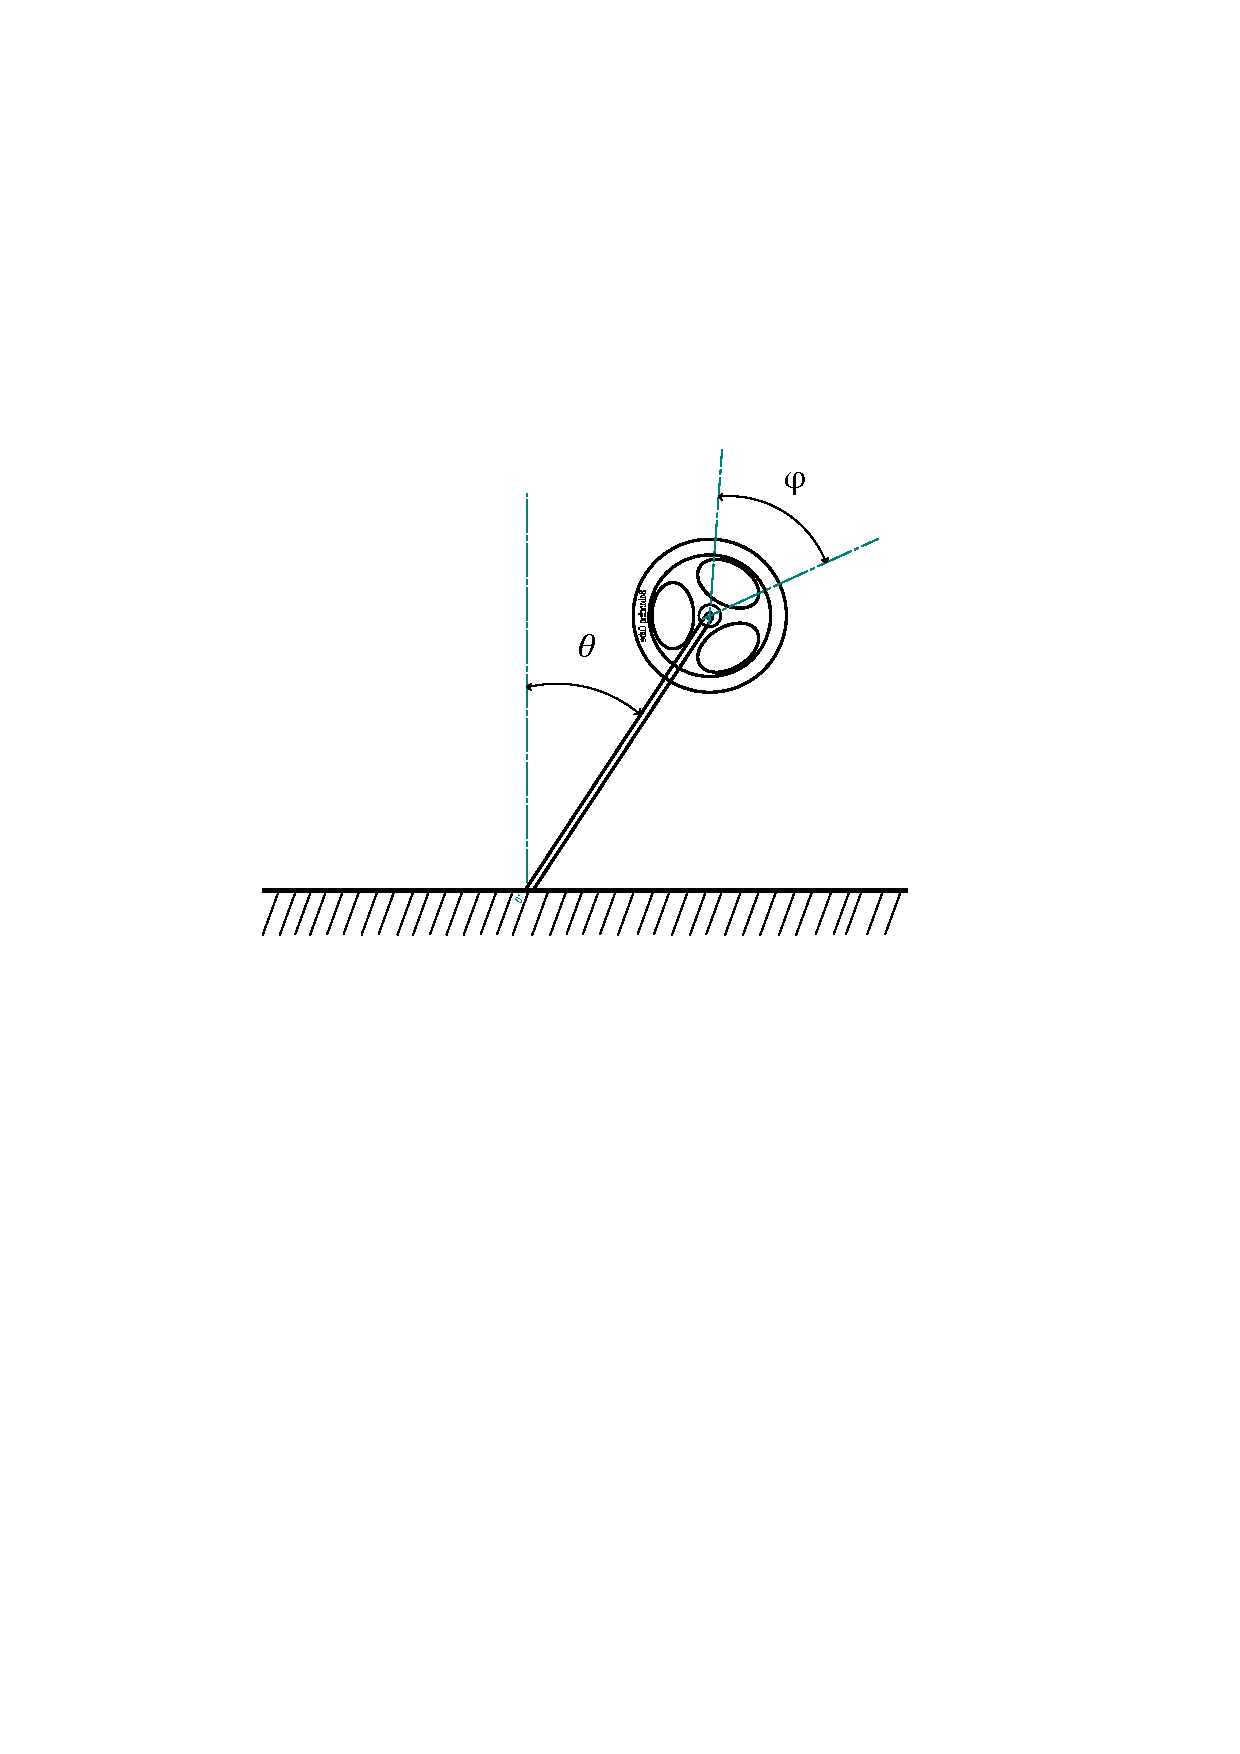
\includegraphics[scale=.6]{Lagrangeflywheel.pdf}
\caption{Cube modelled as a reaction wheel pendulum}
\label{fig:Lagrangeflywheel}
\end{figure}

\emph{Lagrangian} Dynamics have been used to derive the systems behaviour. Firstly by expressing the generlized forces, the energy functions and lagrangian. And then acquire the equations of motion from the Lagrange equation  \cite{Lagrangeref}. Consider the Lagrangian equation

\begin{equation}
\tau_i=\frac{d}{dt}\left(\frac{\partial \mathcal{L}}{\partial \dot{q_i}}\right)-\left(\frac{\partial \mathcal{L}}{\partial q_i}\right)
\end{equation}

Where $\tau$ is generilzed force, in this case a torque. The cube's angular momentum is counteracted by the flywheel and the system can be divided into two parts, One considering the movement of the cube, the other the flywheel.

\begin{equation} \label{eq:positiveL}
\tau_k=\frac{d}{dt}\left(\frac{\partial \mathcal{L}}{\partial \dot{\theta}}\right)-\left(\frac{\partial \mathcal{L}}{\partial \theta}\right)
\end{equation}

\begin{equation} \label{eq:negativeL}
-\tau_k=\frac{d}{dt}\left(\frac{\partial \mathcal{L}}{\partial \dot{\phi}}\right)-\left(\frac{\partial \mathcal{L}}{\partial \phi}\right)
\end{equation}

Whereas $\theta$ represents the angle of the cube and $\phi$ is the position of the flywheel. \\
The Lagrange equation is derived from the difference in kinetic energy and potential energy of the cube

\begin{equation} \label{eq:Lagrange}
\mathcal{L} = E_k - E_p
\end{equation}

\begin{equation} \label{eq:kinetic energy}
E_k = \frac{I_c \cdot \dot{\theta^2}}{2} + \frac{I_f \cdot \dot{\phi^2} }{2}
\end{equation}

\begin{equation} \label{eq:potential energy}
E_p = \frac{M_c \cdot g \cdot l \cdot \cos \theta}{\sqrt{2}}
\end{equation}
The lagrangian \eqref{eq:Lagrange} is then

\begin{equation}
\mathcal{L} = \frac{I_c \cdot \dot{\theta^2}}{2} + \frac{I_f \cdot \dot{\phi^2} }{2} - \frac{M_c \cdot g \cdot l \cdot \cos \theta}{\sqrt{2}} 
\end{equation}

The kinetic energy depends on the angular velocities of the cube construction as well as the flywheel fixed to the motor. Note that the total moment of inertia $I_c$ is defined around the pivot point of the cube. The potential energy has been defined as being at its maximum when the cube is balancing in an upright position. The construction is considered to be symmetric and hence the gravitational force is applied on the center of the cube.
Equation \eqref{eq:positiveL} and \eqref{eq:negativeL} with \eqref{eq:Lagrange}

\begin{equation} \label{eq:negativeL2}
I_c \cdot \ddot{\theta} + \frac{M_c \cdot g \cdot l \cdot \sin \theta }{\sqrt{2}}  = -\tau_k
\end{equation}

\begin{equation} \label{eq:postiveL2}
I_s \cdot \ddot{\phi} = \tau_k
\end{equation}

From these equations it is evident that $\tau_k$ is the torque executed on the flywheel which is wielded by the motor torque $\tau_m$, it can be described by a relation between the torque constant and the current flowing through the motor.

\begin{equation}
\tau_m = K_t \cdot i_m
\end{equation}

The current can be described by the voltage across the two poles of the motor.

\begin{equation} \label{eq:motor torque}
\tau_m = K_t \cdot \frac{U-E_{\text{emf}} }{R_m}
\end{equation}

Note that the motor inductance in neglected in equation \eqref{eq:motor torque}, that is due to the time constant which is fast considering the rest of the system and is not vital for the control system \cite{KTHpendulum}.
The induced voltage can be described as a function of motor speed.

\begin{equation}
E_{\text{emf}} = K_{\text{emf}} \cdot \dot{\phi_r}
\end{equation}

\begin{equation}
\phi_r = \dot{\phi} - \dot{\theta}
\end{equation}
 
\begin{equation} \label{eq:tau}
\tau_m = \frac{K_t}{R_m} U - \frac{K_t K_{\text{emf}} }{R_m} \dot{\phi} + \frac{K_t K_{\text{emf}} }{R_m} \dot{\theta}
\end{equation}

The torque executed on the flywheel can then be described with the torque on the motor shaft, efficiency and gearing. \\ \textsc{Not completely finished with the part below}
\begin{equation} \label{eq:eff}
\tau_k = \tau_m \cdot \eta_m \cdot \eta_g \cdot u
\end{equation}
Based on equation \eqref{eq:negativeL}, \eqref{eq:positiveL} and \eqref{eq:eff} the system can be described by
\begin{equation}
\ddot{\theta} = -\frac{K_t \eta_m}{R_m I_c} U + \frac{K_t K_{\text{emf}} \eta_m}{R_m I_c} \dot{\phi} - \frac{K_t K_{\text{emf}} \eta_m}{R_m I_c} \dot{\theta} - \frac{Mt g l }{\sqrt{2} I_c} \sin \theta \label{thetadotdot}
\end{equation}
\begin{equation}
\ddot{\phi} = \frac{K_t \eta_m}{R_m I_f} U + \frac{K_t K_{\text{emf}} \eta_m}{R_m I_f} \dot{\phi} - \frac{K_t K_{\text{emf}} \eta_m}{R_m I_f} \dot{\theta} 
\label{phidotdot}
\end{equation} 
To use linear control methods the model has to be linearised. This is done at the instable equilibrium where the cube is balancing. Consider the sinus term at the equilibrium point where $\theta$ equals $0$. The term can then be expressed with taylor/macloaruin expansion

\begin{equation} \label{eq: sinus taylor}
sin \theta = \theta - \frac{\theta^3}{3!} +\frac{\theta^5}{5!}... \approx \theta 
\end{equation}

With the equations \eqref{thetadotdot} and \eqref{phidotdot} the system can be described with a state space model with a states $x^T = [\theta, \dot{\theta}, \dot{\phi}$]. The system is hence described by
\begin{equation}
\dot{x} = Ax + Bu
\end{equation} 
where \\
\begin{center}
$\textbf{A} =\begin{bmatrix}
0 & 1 & 0 \\
-\dfrac{Mt g l }{\sqrt{2} I_c} & - \dfrac{K_t K_{\text{emf}} \eta_m}{R_m I_c} & \dfrac{K_t K_{\text{emf}} \eta_m}{R_m I_c} \\ 
0 & \dfrac{K_t K_{\text{emf}} \eta_m}{R_m I_f} & -\dfrac{K_t K_{\text{emf}} \eta_m}{R_m I_f}
\end{bmatrix}$

$\textbf{B} = \begin{bmatrix}
0 \\ 
-\dfrac{K_t \eta_m}{R_m I_c} \\
\dfrac{K_t \eta_m}{R_m I_f}
\end{bmatrix} $
\end{center}
 
\section{Control theory and pole placement}
When using a state-space control system the poles of the controller is chosen by the engineer. But if a poor choice
is made the response of the system will not satisfy the requirements of the regulator. If place to far away from the 
openloop poles high input signals might be required \cite{regler}. The openloop poles can be calculated by solving the eigenvalues 
for the A matrix. Also one must check that the system is controllable for the posed states. Then a gain matrix can 
be computed and the system can be closed.

\section{Pulse Width Modulation}
Pulse Width Modulation:
According to en.wikipedia.org: "Pulse-width modulation (PWM) [...] is a technique used to encode a message into a 
pulsing signal."
This is useful in many power applications, from dimming LED's to motor control. The idea of 
PWM is to alter the voltage over a device while still only having a set level voltage to supply. Simplified  
the voltage is cut into a square wave. This is done by using two transistors, one that can short the motor poles and one that distributes the supply voltage to be applied to the motor \cite{elektro}. If these transistors are switched on and of fast 
compared to the time constant of the motor, the root mean square (RMS) voltage will be the acting voltage.
This allows for a DC voltage that is perceived as lower than the acual supply voltage.
They duty cycle can be changed during operation unlike liner type voltage regulators. 
 
\chapter{Demonstrator}

\textsc{"Nuts"}

\section{Problem Formulation}
The construction of the cube can be seen as the engineering problem. The cube should be a robot that,
using a reaction wheel can balance on its edge. All components were to be mounted in the robot, then only 
requiring a power source. The main componets was a frame, reaction wheel. motor, motor controller, arduino, IMU, 
and encoder.  

The main goal of this project was to build a structure which remain stable in an unstable condition. A process of this sort can be divided into several parts. 
\begin{itemize}
\item Construction
\item Motor Control
\item Sensor Reading
\item System Control
\item Final Assembly
\end{itemize}
All these individual system had to be implemented and joined in the final assembly.
\section{Model validation}
To synthesize a mathematical model from a real world problem it's often beneficial to simplify the reality. Examples of assumption made for this application would be that center of mass is located at the center of the cube, the friction in the motor is ignored and the frame is considered stiff etcetera. 
To validate the model from chapter \ref{chapter: state space}, events with known results can be tested. To do so, Simulink \cite{MATLAB:2014} is used.
First of all the DC-motor model is validated to known characteristics, such as no load speed and current. 

\begin{figure}[!htb] 
\centering
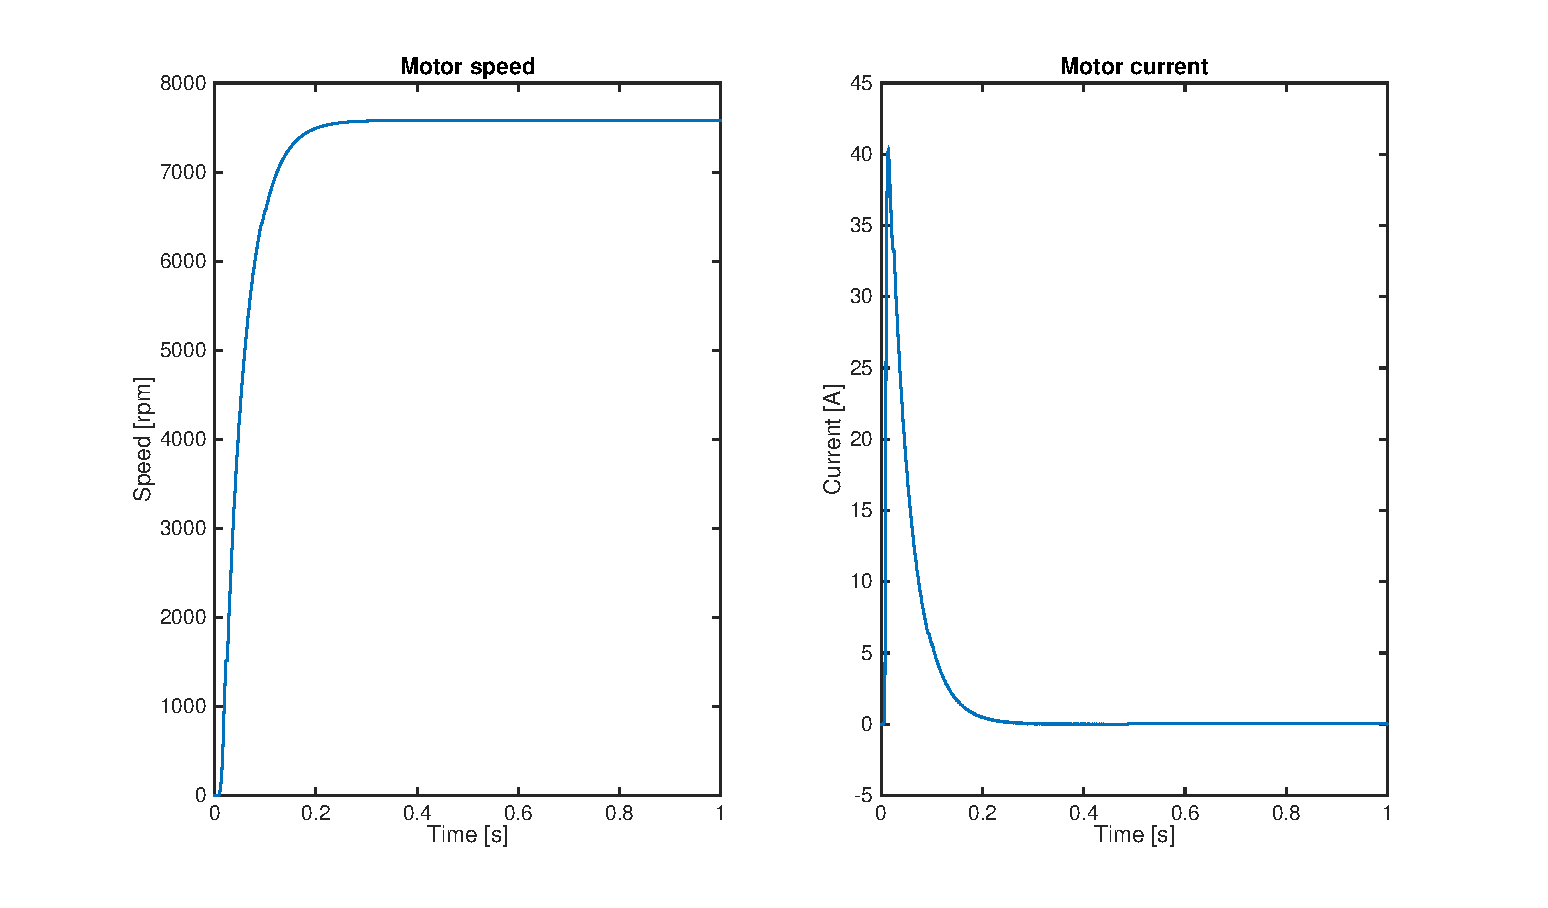
\includegraphics[width = \textwidth]{Motor_noload.eps}
\caption{Validation of motor model}
\label{fig:Motor noload}
\end{figure}

The graphs in figure \ref{fig:Motor noload} displays the speed and current of the unloaded motor. Showing that the motor model correlates with the specified speed and current of an unloaded motor.

The dynamics of the cube is simplified as an inverted pendulum. That means if there is no control input to the system it should behave as pendulum in free movement. That is, it should oscillate at a constant amplitude. As there is no torque applied to the flywheel rotor should be static at all times.

\section{Inertial navigation system}

\subsection{Kalman implementation}
For the implementation of Kalman filter a library made by Lauszus was used, which is available a the Github repository\cite{TKJkalman}. For an extended explanation of the Kalman implementation, see appendix \ref{app: Kalman imp}.

\begin{figure}[!htb]
\centering
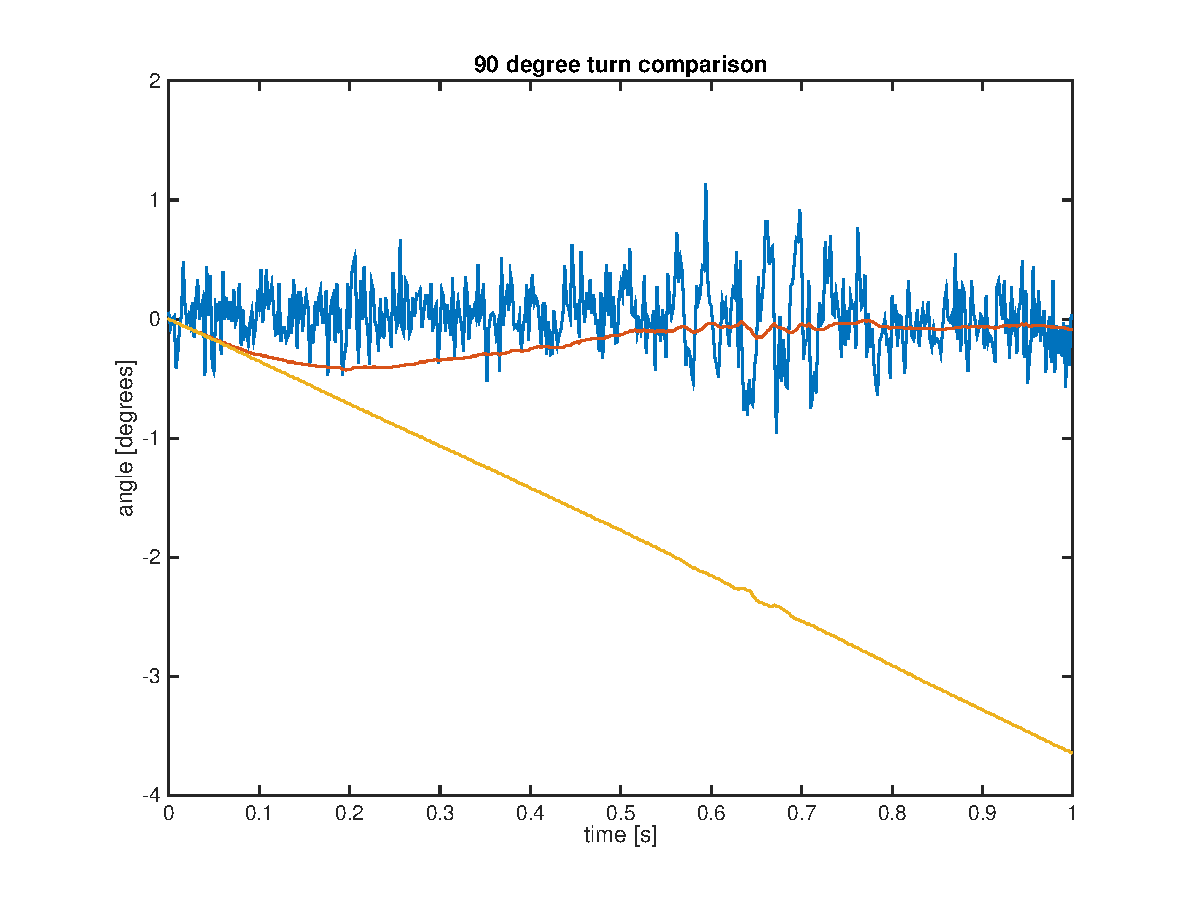
\includegraphics[width = \textwidth]{Kalmancomparisonstat.eps}
\caption{Comparison of Kalman filtered signal and original signal (TO BE UPDATED)}
\label{Fig: Kalman comparison}
\end{figure}

Figure \ref{Fig: Kalman comparison} shows a comparison of the estimated angle at a stationary position using the gyroscope, accelerometer and the Kalman filtered signals separately. The estimated angle using only the gyroscope can be seen by the negative angle ramp. This is due to the bias that is being integrated. The accelerometer readings show that the signal contains a lot of white noise but still has a mean value of zero. 
The Kalman filtered angle starts following the gyroscope readings but are then corrected when weighed against the accelerometer measurements which can be seen early in the plot. 
This indicates that the Kalman filter works as it should but the estimated state should still not be considered \textit{true} as the reference is zero. 


\begin{figure}
\centering
\begin{subfigure}{.5\textwidth}
  \centering
  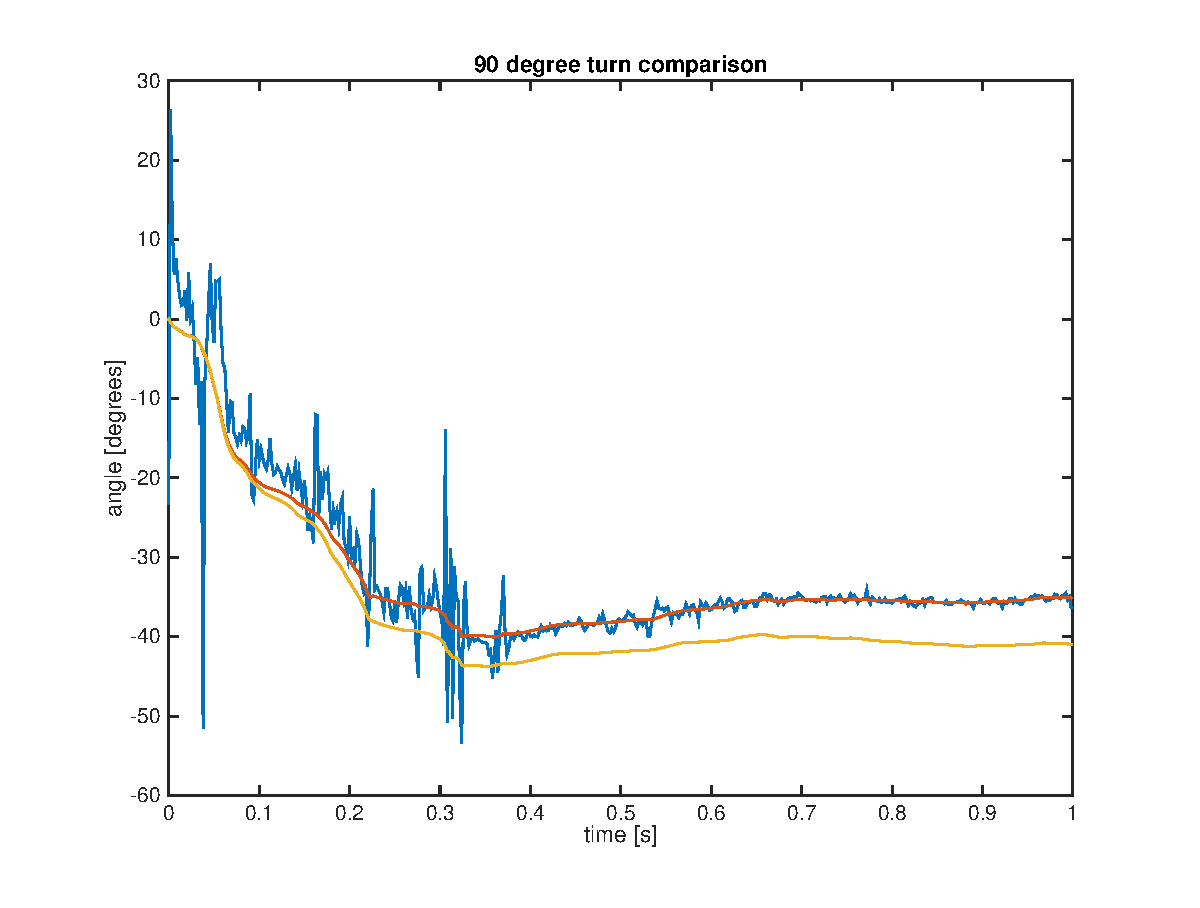
\includegraphics[width=\textwidth]{Kalmancomparisonturn.eps}
  \caption{90 degree turn}
  \label{Fig: Kalmanturn}
\end{subfigure}%
\begin{subfigure}{.5\textwidth}
  \centering
  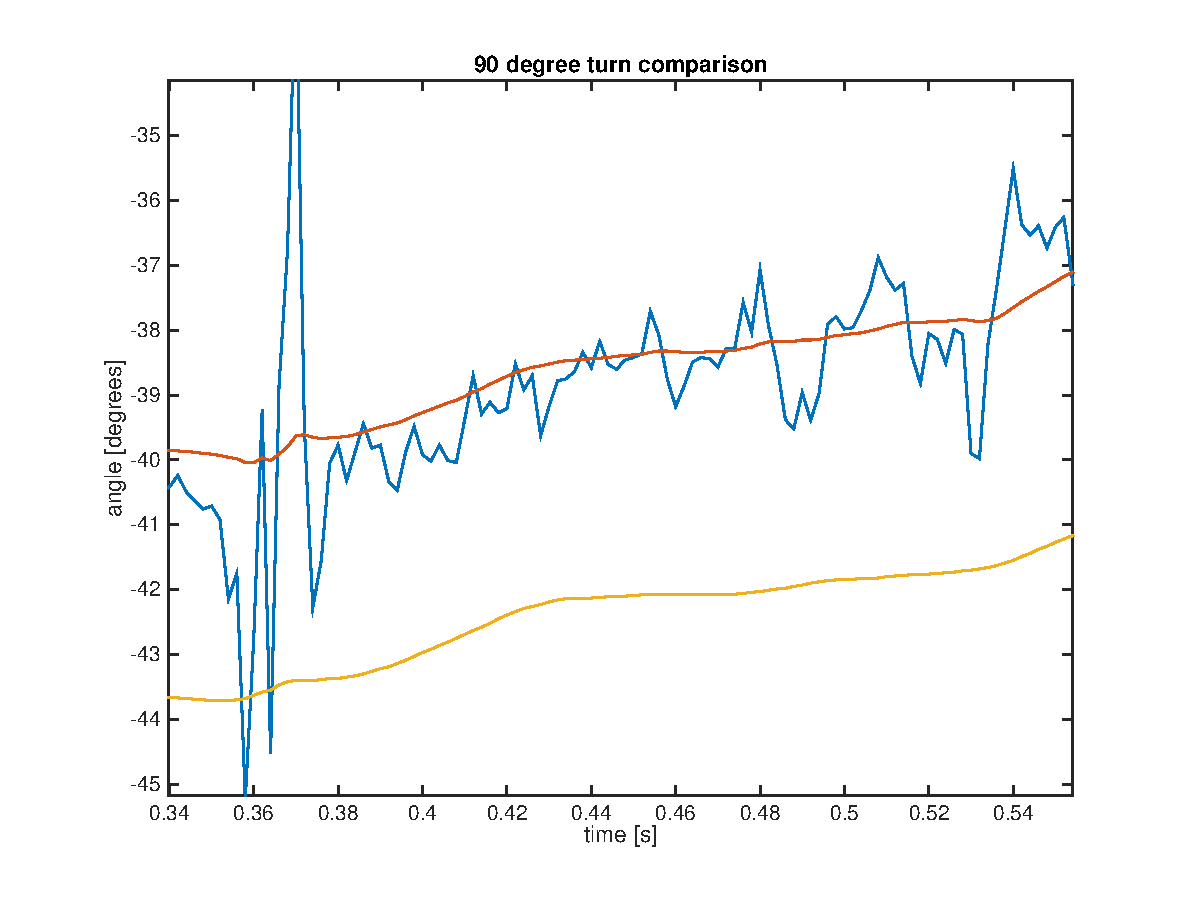
\includegraphics[width=\textwidth]{Kalmancomparisonturnzoom.eps}
  \caption{Zoomed view}
  \label{Fig: Kalmanturnzoom}
\end{subfigure}
\caption{A figure with two subfigures}
\label{Fig: Kalmanturnfull}
\end{figure}

Figure \ref{Fig: Kalmanturnfull} illustrates the estimated angle during a 90 degree turn done by hand. Subfigure \ref{Fig: Kalmanturnzoom} shows a zoomed view of the plot where the gyroscope bias is obvious but the Kalman angle still follows the true value \textbf{Säger jag emot mig sj ? ,...} .



\subsection{Measurement and process noise} \label{chapter:Allan Variance}
For the Kalman filter to properly work it is essential to know how reliable the process and measurement inputs are.  A way of determining the process noise and measurement noise of the IMU is the Allan variance method. The theory of Allan variance is outside the scope of this thesis but for reader reference is a time domain analysis technique commonly used to determine the characteristics of errors for inertial sensors\cite{Allancalibration}.
The gyroscope data is treated as an external input to the system, so the error and bias from the readings are characterised as process noise. This is then compared to the measurement, the accelerometer, which contains a measurement noise.
By gathering samples from the gyroscope and accelerometer at a stationary state the Allan variance can be calculated. The Allan variance is then used to determine the noise and stability of the system. The interesting components of the variance for the IMU are the ARW, VRV and bias stability mentioned in section \ref{section:IMU}.
Data from the gyroscope were collected during twelve hours to \textbf{achieve, ordval?} a reliable estimate of the bias. 
The root Allan variance was calculated and is shown in Figure \ref{fig:gyroscope allan} where the variance is a function of averaging time $\tau$

\begin{figure}[!htb]
\centering
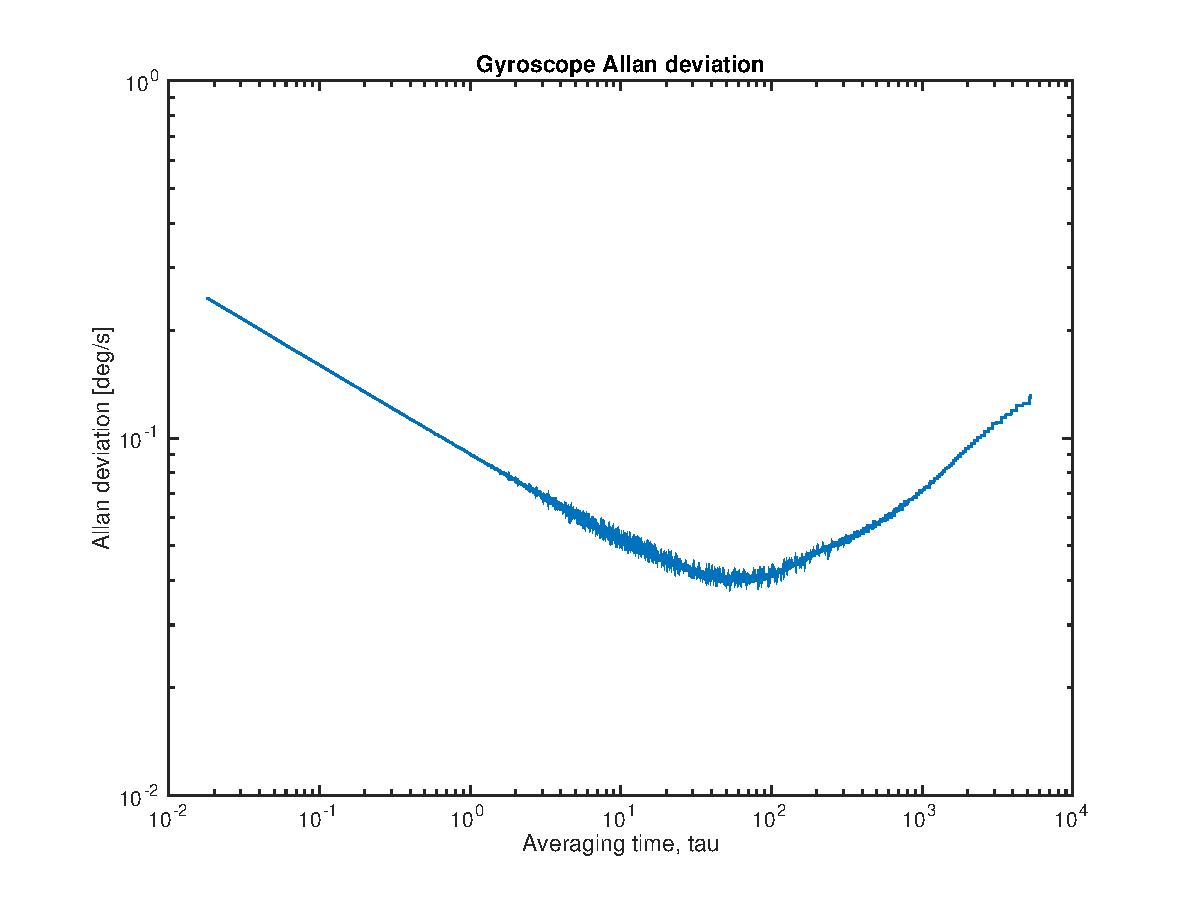
\includegraphics[scale=.7]{gyroscopeallan.eps}
\caption{Gyroscope root Allan variance \textsc{fix pic}}
\label{fig:gyroscope allan}
\end{figure}

The angle (or velocity, concerning the accelerometer) random walk can be depicted from the plot at an angle of -0.5 while the bias instability is determined by looking at the lowest point of the plot. Allan variance for the accelerometer was \textbf{framtagen} in a similar manner.  The results can be seen in table \ref{Table: Allan variance}.

\begin{table}[!hbt]
\centering
    \begin{tabular}{| l | l |} \hline
    Noise term & Degrees/second \\ \hline
    Angle random walk & ARW res \\ \hline
    Bias stability & BS res \\ \hline
    Velocity random walk & VRW res \\
    \hline
    \end{tabular}
    \caption{Allan variance results}
    \label{Table: Allan variance}
\end{table}

These values corresponds to the process and measurement noise covariance matrices used by the Kalman filter. \textbf{Dessa finns bara i appendix ??} 

\section{Software}
To develop and improve a system such as this is an iterative process. To verify changes and improvements in realtime, the model were simulated with Simulink\textsuperscript{\textregistered}. 
%\begin{figure}[!htb]
%\centering
%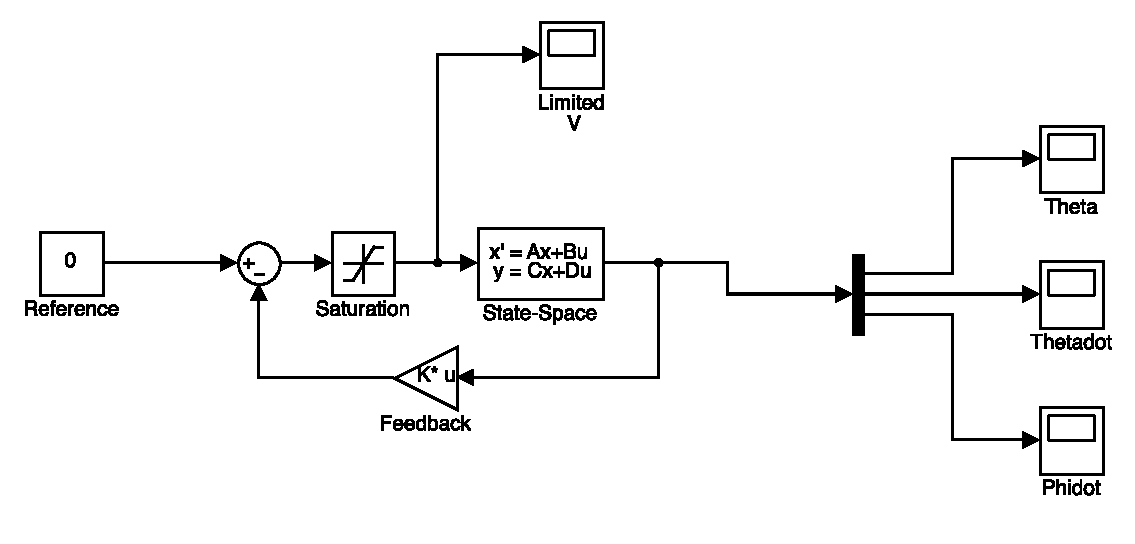
\includegraphics[scale=.7]{simmodel.eps}
%\caption{Simulink model.}
%\label{fig:simmodel}
%\end{figure}



The Simulinkmodel seen in figure \ref{fig:simmodel} describes the system
\\ Something about the  optimizing of the feedback control
\begin{figure}[!htb]
\centering
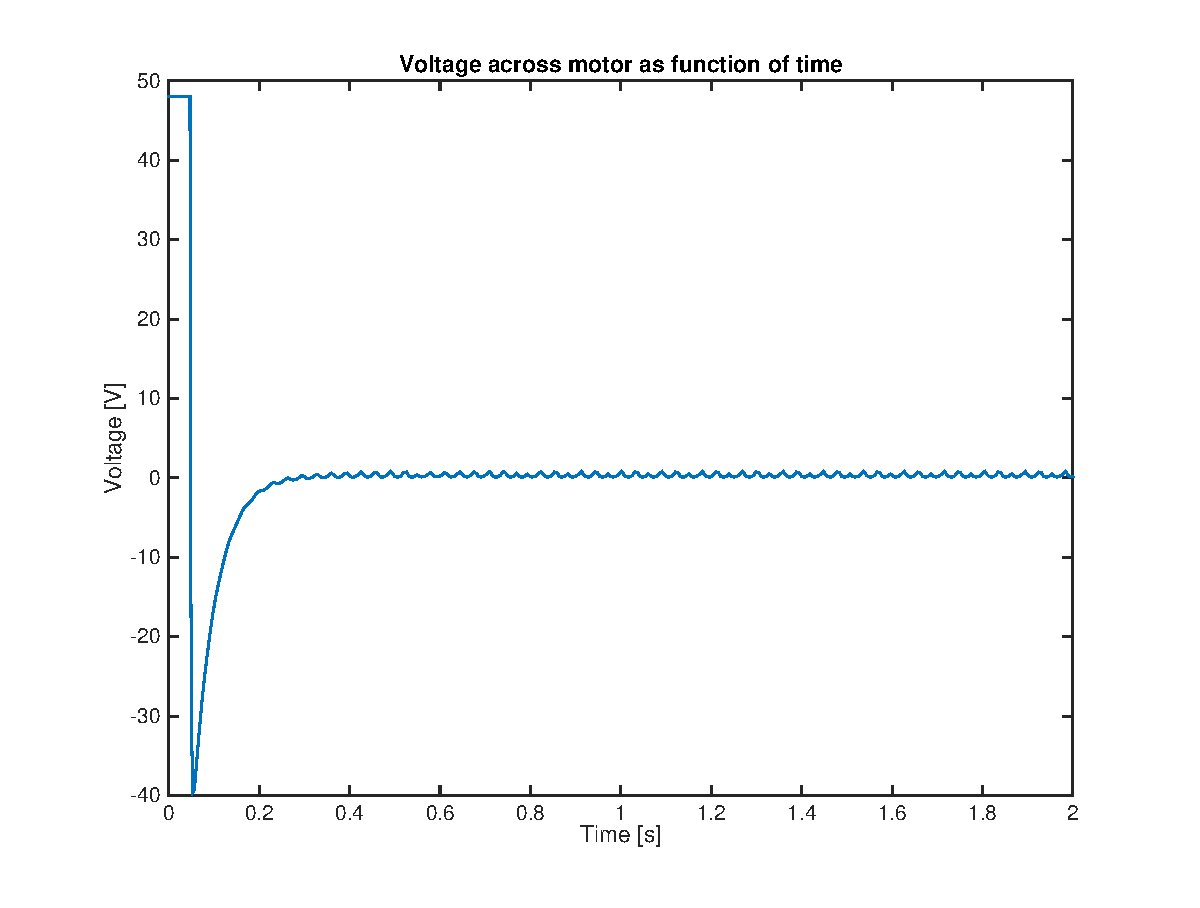
\includegraphics[scale=.7]{voltageplot.eps}
\caption{Voltage across motor poles.}
\label{fig:voltageplot}
\end{figure}

The voltage supplied to the motor

\begin{figure}[!htb]
\centering
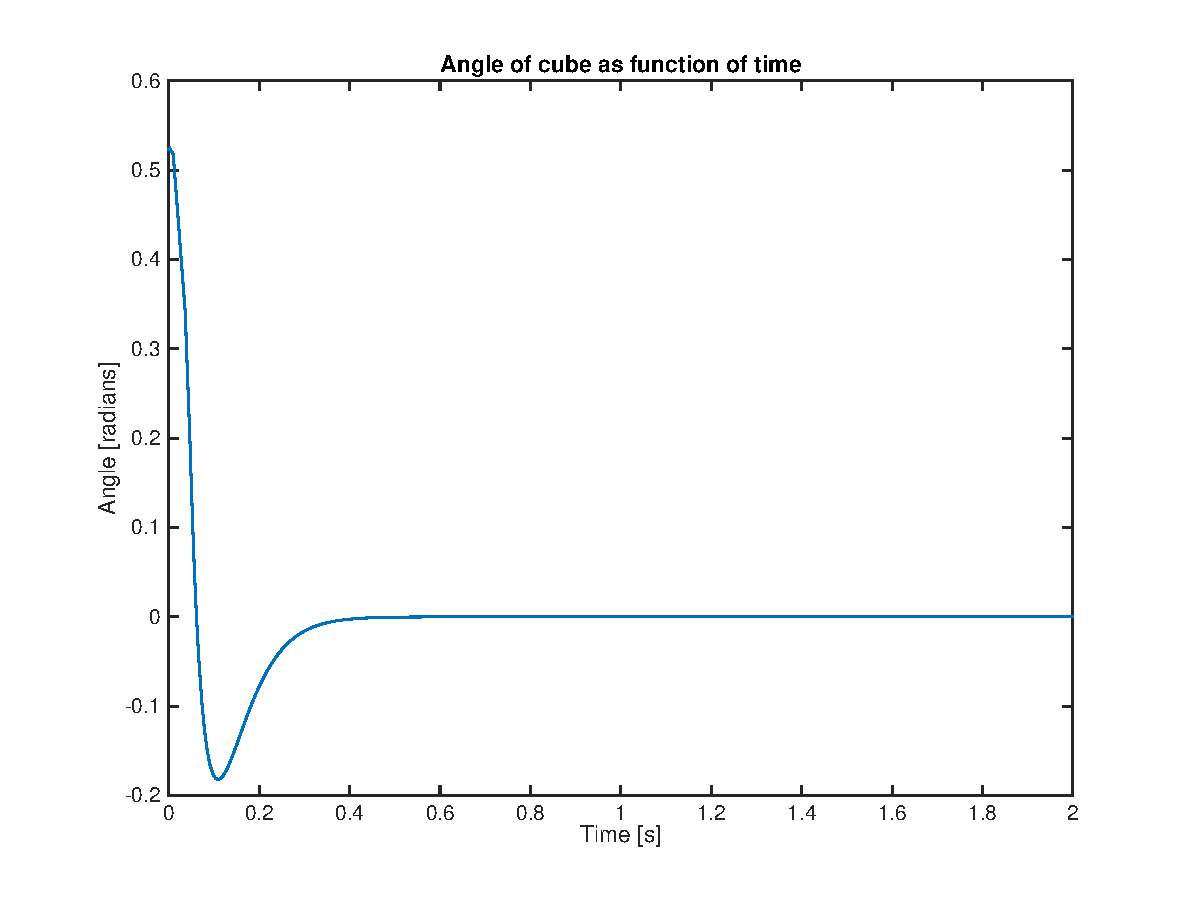
\includegraphics[scale=.7]{angleplot.eps}
\caption{Angle of the cube.}
\label{fig:voltageplot}
\end{figure}

The angle of the cube. Very good such magic


\section{Electronics}
Beskriv din elektroniska konstruktion. Använd figurer och förenklade blockschema. Motivera dina lösningar.
How do we send data?
\\ Sensors
\\ Motor
\\ Arduino
\\ Motor control

\subsection{PWM}
The PWM frequency were chosen to 20KHz, the maximum the motor controler can cope with [].
 

\subsection{System Control}
The choosen control method where state space. The problem in to linareise and discretise with good enough precition.The poles for the control system were choosen for the openloop system and the system was simulated in 
	simulink to assure that the respose was as expected. 
	The gain matrix is calculated as the eigenvalues of A-BK ~= p, (p is the choosen poles), using matlab place
	It uses a robust calculation algorithm formulated by Kautskyn for determining the gain matrix.


To be able to use a microcontroler the controlsystem must be discrerte. When translating a analytical system to a 
discrete system a few thing must be considerd. The method of samplig is crutial. If the sampling frequancy is to 
low the system responce might not detct changes att all or aliasing can cause it to behave unexpectedly. Due to the 
Nyquist critera the sampling frequency mus be: f>=2*t, twice as high as the smalles frequency you want to be able to
detect. Then the signal must be low pass filterd with a cut off frequecny close to t to make sure that no unwanted
frequencies is taken into the regulator.
All non measured derivatives must be calculated. Simulink does this by calculatin an combination of tustin and 
backward Euler[mathworks][bilaga]. This causes a numerical error depending on the step in time. And the time step
in turn depends on the sampling frequency, too low frequency causes a big stem in time which leads to large numerical 
errors.
Most variables and states will in the microprocessor be handels as double or also know an Double-point floating-point
format. This causes an trunctuation error in every calculation. The double is only the size of a float, 32-bit(?). This
means that we unly reliably can use 6 decimal digits of precition[float].

\section{Hardware}
The motor is fixed through the middle wall in the cube, the shaft on one side and the body on the other. The flywheel is dicrectly mounted to the motor shaft. All other components are mounted on the motor-body side of the cube.
\\ Basic construction

\subsection{Construction}
The main construction problem where deciding the size of the cube and reaction wheel. A too big reaction wheel for the motor has a large affect on the cubes ability to balance. The problem were (uppställt) with Newtonian mechanics.
Also idealy the cube should be nice looking, easy to produce and simple to assemble. 
 
\subsection{Motor and Motor Control}
The motors nominal and stall torque are very important for the system blaha. The motor driver is also important, but usually one can get suggestions on drivers from motor manufactures, which was the chosen path.
  
\subsection{Sensor Reading}
The IMU's parameters and filtering of the signals

\subsection{Final Assembly}
When the subproblems above are solved and constructed, the final machine can be built. Here cabling and disturbances from other subsystems must be taken into consideration. 
The IMU placement would provisoricly be tried to se a placement were bad due to more disturbances form other compunents i.e. netsupply and motor lining.





\chapter{Results}
Beskriv resultatet. 

\chapter{Discussion and conclusions}
\emph{I detta kapitel diskuteras och sammanfattas de resultat som presenterats i föregående kapitel. Sammanfattningen baseras på en resultatanalys och syftar till att svara på den fråga eller de frågor som formuleras i kapitel i.}

The IMU measures very small voltage alterations when the capacitance varies in the mechanical system. Placing such a sensitive device near a motor which induces a flow of bla bla bla

\section{Discussion}
Motor choice osv

\section{Conclusions}
Successful victory


\chapter{Recommendations and future work}

\section{Recommendations}
A more extensive research with non-linear control systems has been done at ETH, with the name Cubli,\cite{cubliECC13}

\section{Future work}
An extension of the project would be balancing the cube not only on it's edge but it's corner. To achieve this multiple reaction wheels must be used and a more complicated control system due to changes in moment of inertia caused by angular velocities in the other reaction wheels.

%\bibliography
\cleardoublepage
\bibliography{FiM_references}
\bibliographystyle{apalike-url}%apalike-url}

\cleardoublepage
\appendix
\addtocontents{toc}{\protect\contentsline {part}{Appendices}{}{}}


\chapter{Additional information} \label{appA}
\section{Elaborative Kalman explanation (TITLE?)} \label{app: Kalman}
\subsection{Mathematical background}
To understand this recursive filter which use old and new values a \textit{a priori} and \textit{a posteriori} state is defined
\begin{equation} \label{eq: priori state}
\hat{x}^-_k
\end{equation}
\begin{equation} \label{eq: posteriori state}
\hat{x}_k
\end{equation}
The \textit{a priori}  state in equation \eqref{eq: priori state} is defined as the estimate of the current state at the time $k$. The \textit{a posteriori} state \eqref{eq: posteriori state} is the new estimated state.
For the Kalman filter to work properly some criteria has to be fulfilled. The average value of the measurement noise $z$ and process noise $w$ has to be zero, i.e. a Gaussian error. $z$ and $w$ also has to be independent of  each other. The noise and error in an IMU and many other devices have the characteristics of Gaussian noise.




During the \textit{predict} phase the filter estimates the states using the inputs from the process, i.e the gyroscope. It then moves on to the \textit{update} phase where it compares the state to the actual measurement, the accelerometer. See Figure \ref{Fig: Kalman phases}.
Consider the true state equation \eqref{eq:kalmanstate}, the Kalman filter is firstly estimating the first state by neglecting the process noise
\begin{equation} \label{eq:Kalman first estimate}
\hat{x}^-_k = A\hat{x}\textsubscript{k-1}+Bu\textsubscript{k-1}
\end{equation}
As stated above the Kalman filter uses readings from both the gyroscope and accelerometer to estimate a position closer to the true value. To determine how reliable the process and measurement readings are a noise covariance is defined as
\begin{equation} \label{eq:covariance process noise}
Q = E(w_k w_k \textsuperscript{T})
\end{equation}
\begin{equation} \label{eq:covariance measurement noise}
R = E(v_k v_k \textsuperscript{T} )
\end{equation}
How to determine these covariances are further investigated in section  \ref{chapter:Allan Variance}
From here the \textit{a priori} error covariance matrix is introduced to symbolize the noise in the process measurement
\begin{equation}
P^-_k = AP\textsubscript{k-1}A^T + Q_k
\end{equation}
During the \textit{update} the accelerometer measures are used. The measurement \textit{innovation} is calculated as
\begin{equation} \label{eq: innovation}
\tilde{y} = z_k - H\hat{x}^-_k
\end{equation}
The \textit{innovation} is a residual that reflects the relation between the predicted measurement and the actual measurement. A measurement \textit{innovation} of zero indicates a perfect agreement.
The measurement \textit{innovation} covariance is calculated as
\begin{equation} \label{eq:innovation cov}
S_k = HP^-_kH^T + R
\end{equation}
The \textit{innovation} covariance is very similiar to the \textit{priori} error covariance but represents the measurement instead. From here the core of the Kalman filter can be calculated, the Kalman gain
\begin{equation} \label{eq:Kalman gain}
K_k = P^-_kH^TS\textsuperscript{-1}_k
\end{equation}
indicates how reliable the measurement is. Note that if the measurement covariance error \eqref{eq:covariance measurement noise} is large the Kalman gain will be small and vice versa if the \textit{priori} error covariance is large.
By now the \textit{posteriori} state can be estimated by
\begin{equation}
\hat{x}_k = \hat{x}^-_k + K_k\tilde{y}_k
\end{equation}
A current state has been estimated and the Kalman filter and finally the \textit{priori} error covariance is updated
\begin{equation}
P_k=(I-K_kH)P^-_k
\end{equation} 
The filter now returns to the measurement phase seen in figure \ref{Fig: Kalman phases}.
For further reading, and mathematical proof see \cite{Kalmanintro}.


\subsection{Implementation}
\label{app: Kalman imp}
The Kalman filter cycles two states, the \textit{predict} and \textit{update} phases. Kalman is using discretized steps making the filter implemented on a microprocessor fairly simple. 
An implementation of the Kalman filter on the IMU would look something like this

Consider the equation \eqref{eq:Kalman first estimate} from chapter \ref{app: Kalman} . At first the filter predicts the state
\begin{equation}
\hat{x}^-_k = A\hat{x}\textsubscript{k-1}+Bu\textsubscript{k-1}
\end{equation}

Where

\begin{equation}
\textbf{x}_k = \begin{bmatrix}
\theta \\
\dot{\theta_b}
\end{bmatrix}_k
u\textsubscript{k-1} = \dot{\theta}
\end{equation}

\begin{equation}
\textbf{A} = \begin{bmatrix}
1  & -\Delta t \\
0   & 1
\end{bmatrix}
,
\textbf{B} = \begin{bmatrix}
\Delta t \\ 0
\end{bmatrix}
\end{equation}

The states used here  are the angle as well as the bias. Next up is the \textit{priori} error covariance
\begin{equation}
P^-_k = AP\textsubscript{k-1}A^T + Q_k
\end{equation}

\begin{equation}
\begin{bmatrix}
P\textsubscript{11} & P\textsubscript{12} \\
P\textsubscript{21} & P\textsubscript{22}
\end{bmatrix}^-\textsubscript{k} =
\begin{bmatrix}
1  & -\Delta t \\
0   & 1
\end{bmatrix}
\begin{bmatrix}
P\textsubscript{11} & P\textsubscript{12} \\
P\textsubscript{21} & P\textsubscript{22}
\end{bmatrix}\textsubscript{k-1}
\begin{bmatrix}
1 & 0 \\
-\Delta t & 1
\end{bmatrix}
+
\begin{bmatrix}
Q\textsubscript{ $\theta$ } & 0 \\
0 & Q\textsubscript{$\dot{\theta}_b$}
\end{bmatrix}
\Delta t
\end{equation}

The innovation covariance mentioned in \ref{eq:innovation cov}

\begin{equation} 
S_k=
\begin{bmatrix}
1 & 0
\end{bmatrix}
\begin{bmatrix}
P_{11} & P_{12} \\
P_{21} & P_{22} 
\end{bmatrix}^- _k
\begin{bmatrix}
1 \\ 0
\end{bmatrix}
+
R
\end{equation}
Kalman gain
\begin{equation}
\begin{bmatrix}
K_1 \\ K_2
\end{bmatrix}_k
=
\begin{bmatrix}
P_{11} & P_{12} \\
P_{21} & P_{22}
\end{bmatrix}^-_k
\begin{bmatrix}
1 \\ 0
\end{bmatrix}
S^{-1}_k
\end{equation}

The predicted states are then updated with the \textsc{weighed} measures from the accelerometer

\begin{equation}
\begin{bmatrix}
\theta \\
\dot{\theta_b}
\end{bmatrix}_k
=
\begin{bmatrix}
\theta \\
\dot{\theta_b}
\end{bmatrix}_k^-
+
\begin{bmatrix}
K_1 \\ K_2
\end{bmatrix}_k
\textbf{$\tilde{y}$}
\end{equation}

And then at last the error covariance

\begin{equation}
\begin{bmatrix}
P\textsubscript{11} & P\textsubscript{12} \\
P\textsubscript{21} & P\textsubscript{22}
\end{bmatrix}\textsubscript{k} 
=(
 \begin{bmatrix}
1 & 0 \\
0 & 1
\end{bmatrix}
-
\begin{bmatrix}
K_1 \\ K_2
\end{bmatrix}_k
\begin{bmatrix}
1 & 0
\end{bmatrix}
)
\begin{bmatrix}
P\textsubscript{11} & P\textsubscript{12} \\
P\textsubscript{21} & P\textsubscript{22}
\end{bmatrix}^-\textsubscript{k}
\end{equation}


This is done during each loop of the microcontroller to ensure that the estimated state is as near the true state as possible.

\section{Arduino PWM implementation} \label{app: PWM}
The arduino micro controler has a couple of different standard pulse width modulation (\textit{PWM} modes. But the standard frequencies are 490 and 980 Hz. "Having" a significantly higher 
frequency have many advantages, especially for the control system. The chosen motor controller could work in two modes, one of them being ultrasonic the other below ultrasonic. Setting the PWM frequency above the standard frequency is preferably because the the motor becomes more efficient \textsc{SOURCE} and the human ear can not hear frequencies above ~ 18 KHz. The Arduino uno's maximum PWM frequency is ~ 61 KHz, which is too much for the motor controller \textsc{WHY}. A bit of register manipulation had to be 
done to accomplish an acceptable PWM frequency.

The Arduino has 3 clocks that controls various pins and functions in the environment. The clocks, and their respective pins and bit size, are:
\begin{itemize}
\item[\textbf{Timer 0}]
controls digital pin 10 and
works in 8-bits it also used as reference for the delay(), millis() and micros() built in functions. i.e. changing timer 0 might disturb the code up if the code is using these functions. 
\item[\textbf{Timer 1}]
The 16-bit timer. Controlls pin 5 and 6 and has more modes of operation than the other two timers
\item[\textbf{Timer 2}]
another 8-bit timer responsible for pin 3 and 11 on the 
Arduino Uno.
\end{itemize}
Each of these timers can be set the various PWM modes individually, ---more on this later---. All timers have prescalers which divides the chips clock speed to vary the 
frequency of the PWM signal in rough discrete steps (the difference between the fastest and the next to fastest fequency on timer1 is 53 KHz)(see avr documentation for mor info) \textbf{källa h'r eller ??}. 

When using PWM, the PWM duty cycle is used (and optionally frequency). Once the PWM duty cycle is set this works parallel to the main program and does not effect the main program but is rather run \textbf{annan tråd??}(except 
when changing the PWM parameters). For example this is useful when only one Arduino is used for multiple tasks, and computing time becomes expensive. A non inverted mode where used, 
meaning that 100\% duty cycle equals full power all the time. There are multiple modes of PWM on the Arduino. The main ones that can be choose from are fast - and phase corrected PWM. 
When using the phase correct PWM (pcPWM) a counter counts up every clock cycle until the counter reaches a compare value, \textit{TOP}. When TOP is reached the counter is reset or "set" according to the AVR 
documentation, be aware that for the method to work, the counter has to be adjusted to "set" not "clear" or "set bottom". Then the duty cycle has to be set to a value between 0 and TOP. Choosing duty to TOP/2 will yield a 50\% duty cycle. For modes where the TOP value is not specified it defaults to 0xFF or 255 in decimal.

When using the pcPWM (on timer2 in this case), mode 5, the TOP value and duty cycle for ONE of timer2's pin's are the same variable. This means that one can not change the duty 
cycle for a certain frequency. The frequency can then be explained by equation \ref{eq: clock freq}
\begin{equation} \label{eq: clock freq}
frequency = \frac{clock}{2 \cdot prescaler \cdot TOP}
\end{equation}

But the other pin (nr 3) is left uneffected. So if the desired PWM is 20 KHz it is done by choosing 100 
as TOP (OCR2A for timer2) and the prescaler value to 8 (TCCR2B = (1<<CS21) pin 11 will always have 50\% duty cycle at 20 KHz. But the duty cycle for pin 3 can be set continiously.  you can choose another duty cycle for pin 3  \textbf{HÄR ÄR DET KNAS ?}
(OCR2B) while maintaining 10 KHZ due to the TOP, OCR2A value is not changed. The disadvantage of this method is that it requires 2 pins, while only one is used. A minor price to pay for a specific frequency and reduced headache from the high pitched noise.

To choose mode you must set the correct WGM vaues in the TCCR2A and TCCR2B registers. The fourth letter "2" represents timer 2. Timer 2 is 8-bit so it has a maximum of 8 modes. If instead timer 1 is 
used more modes can be chosen allowing for a greater amount of operation modes. Other Arduino boards might have a greater number of timers which allows for more than three different PWM's, with non default frequencies, being used at the same time.

\chapter{Proofs} \label{appB}

\cleardoublepage   
\cleartoverso %force back cover to be "left" page
%
\includepdf[pages={2}]{kth-cover.pdf}

%\printbibliography
\end{document}
